\loai{Định nghĩa nhiệt dung riêng}


\loai{Đặc điểm của nhiệt dung riêng}
\begin{ex}
	Nhiệt dung riêng của đồng là $380 \ J/kg. K$, điều này cho biết
	\choice
	{nhiệt lượng cần thiết để làm cho $1 \ g$ đồng nóng lên thêm $1^\circ C$ là $380 \ J$}
	{nhiệt lượng cần thiết để làm cho 1 khối đồng nóng lên thêm $1^\circ C$ là $380 \ J$}
	{\True nhiệt lượng cần thiết để làm cho $1 \ kg$ đồng nóng lên thêm $1^\circ C$ là $380 \ J$}
	{nhiệt lượng cần thiết để làm cho $1 \ kg$ đồng nóng lên là $380 \ J$}
	\loigiai{
		Nhiệt dung riêng của đồng là $380 \ J/kg. K$ có nghĩa là để tăng nhiệt độ của 1 kg đồng lên thêm $1^\circ C$, cần cung cấp $380$ J nhiệt lượng.
	}
	\haidong{2}\end{ex}
\loai{Đơn vị của nhiệt dung riêng}

\begin{ex} \nguon{2}
	Đơn vị của nhiệt dung riêng là
	\choice
	{\True $J / kg . K$}
	{$J /kg / K$}
	{$K / kg. J$}
	{$kg / J . K$}
	\loigiai{
		Đơn vị của nhiệt dung riêng là $\dfrac{J}{kg . K}$.
	}
\end{ex}

\loai{So sánh nhiệt dung riêng}
\begin{ex} \nguon{2}
	\immini[thm]{Cho nhiệt dung riêng của một số chất ở $0^\circ C$ ở bảng bên. Nếu các chất trên có cùng khối lượng thì chất nào sẽ dễ nóng lên và cũng dễ nguội đi so với các chất còn lại?
		\choice
		{Nhôm}
		{Đồng}
		{\True Chì}
		{Nước đá}
	}{$
		\begin{array}{|l|l|}
			\hline \text { Chất } & \text { Nhiệt dung riêng (J/kg.K) } \\
			\hline \text { Nhôm } & 880 \\
			\hline \text { Đồng } & 380 \\
			\hline \text { Chì } & 126 \\
			\hline \text { Nước đá } & 1800 \\
			\hline
		\end{array}
		$}
	\loigiai{
		Chì có nhiệt dung riêng thấp nhất, do đó nó sẽ dễ nóng lên và cũng dễ nguội đi hơn các chất còn lại khi có cùng khối lượng.
	}
\end{ex}
\loai{Biểu thức tính nhiệt lượng theo nhiệt dung riêng}
\begin{ex}
	Nhiệt lượng cần cung cấp để tăng nhiệt độ của $m \ kg$ vật liệu (có nhiệt dung riêng $c$) từ nhiệt độ $t_1$ lên tới nhiệt độ $t_2$ là
	\choice
	{\True $Q=m c\left(t_2-t_1\right)$}
	{$Q=m c\left(t_2+t_1\right)$}
	{$Q=m c\left(t_2 . t_1\right)$}
	{$Q=m c\left(\dfrac{t_2}{t_1}\right)$}
	\loigiai{
		Nhiệt lượng $Q$ cần cung cấp để tăng nhiệt độ của một khối lượng $m$ vật liệu từ nhiệt độ $t_1$ lên tới nhiệt độ $t_2$ được tính theo công thức:
		\[ Q = mc\Delta t = m c (t_2 - t_1)\] 
		trong đó $c$ là nhiệt dung riêng của vật liệu, $t_2$ là nhiệt độ sau cùng và $t_1$ là nhiệt độ ban đầu.
	}
	\haidong{2}\end{ex}
\begin{ex}
	Trong công thức tính nhiệt lượng thu vào: $Q=mc\Delta t=m c\left(t_2-t_1\right)$, $t_2$ là
	\choice
	{nhiệt độ lúc đầu của vật}
	{\True nhiệt độ lúc sau của vật}
	{thời điểm vật bắt đầu nhận nhiệt lượng}
	{thời điểm sau khi vật nhận nhiệt lượng}
	\loigiai{
		\item Trong công thức $Q=mc\Delta t=m c\left(t_2-t_1\right)$, $t_2$ là nhiệt độ lúc sau của vật, và $t_1$ là nhiệt độ lúc đầu của vật. 
		\item Sự chênh lệch nhiệt độ $\Delta t = t_2 - t_1$ biểu thị sự thay đổi nhiệt độ của vật khi trao đổi nhiệt.
	}
	\haidong{2}\end{ex}
\begin{ex} \nguon{4}
	Độ lớn của nhiệt lượng cần cung cấp cho vật để làm tăng nhiệt độ của vật \textbf{không} phụ thuộc vào
	\choice
	{khối lượng của vật}
	{độ tăng nhiệt độ của vật}
	{tính chất của chất làm vật}
	{\True khối lượng riêng của vật}
	
	\loigiai{
		Khối lượng riêng của vật không ảnh hưởng đến nhiệt lượng cần để tăng nhiệt độ của vật. Nhiệt lượng chỉ phụ thuộc vào khối lượng, độ tăng nhiệt độ và tính chất của chất làm vật.
	}
\end{ex}
\loai{So sánh nhiệt lượng cần làm nóng các vật}
\begin{ex}
	Nhiệt dung riêng của đồng lớn hơn chì. Vì vậy để tăng nhiệt độ của $3 \ kg$ đồng và $3 \ kg$ chì thêm $15^\circ C$ thì
	\choice
	{khối chì cần nhiều nhiệt lượng hơn khối đồng}
	{\True khối đồng cần nhiều nhiệt lượng hơn khối chì}
	{hai khối đều cần nhiệt lượng như nhau}
	{không khẳng định được}
	\loigiai{
		Vì nhiệt dung riêng của đồng lớn hơn chì, nên để tăng nhiệt độ của cùng một khối lượng đồng và chì thêm $15^\circ C$, khối đồng sẽ cần nhiều nhiệt lượng hơn. Sử dụng công thức:
		\[ Q = mc\Delta t \]
		khi $m$ và $\Delta t$ là như nhau, nhiệt lượng $Q$ sẽ phụ thuộc vào $c$ (nhiệt dung riêng).
	}
	\haidong{2}\end{ex}
\begin{ex}
	Có bốn bình $A,\ B,\ C,\ D$ đều đựng nước ở cùng một nhiệt độ với thể tích tương ứng là 1 lít, 2 lít, 3 lít, 4 lít. Sau khi dùng các đèn cồn giống hệt nhau để đun các bình này trong cùng một khoảng thời gian. Bình có nhiệt độ thấp nhất là bình
	\choice
	{A}
	{B}
	{C}
	{\True D}
	\loigiai{
		Do các bình được đun bằng các đèn cồn giống hệt nhau trong cùng một khoảng thời gian, bình có thể tích lớn nhất sẽ có nhiệt độ tăng lên ít nhất vì nhiệt lượng cung cấp được chia sẻ cho khối lượng nước lớn hơn. Vì vậy, bình $D$ (có thể tích lớn nhất 4 lít) sẽ có nhiệt độ thấp nhất.
	}
	\haidong{2}\end{ex}
\begin{ex} \nguon{2}
	Cung cấp nhiệt lượng $Q_1$ cho băng, làm tăng nhiệt độ của khối băng từ $-10^\circ C$ lên $-5^\circ C$. Tuy nhiên ta phải cung cấp nhiệt lượng $Q_2>Q_1$ vào cùng một khối lượng nước ở dạng lỏng để làm tăng nhiệt độ của nó từ $15^\circ C$ lên $20^\circ C$. Từ những kết quả này, bạn có thể kết luận gì?
	\choice 
	{Nhiệt dung riêng của băng lớn hơn của nước} 
	{Cần thêm thông tin để rút ra kết luận}
	{\True Nhiệt dung riêng của băng nhỏ hơn của nước} 
	{Nhiệt dung riêng của băng và nước như nhau}
	\loigiai{
		Vì lượng năng lượng cần thiết để tăng $5^\circ C$ cho băng ít hơn so với lượng năng lượng cần để tăng $5^\circ C$ cho một khối lượng nước bằng nhau, chúng ta kết luận rằng nhiệt dung riêng của băng $c=\dfrac{Q}{m . \Delta T}$ nhỏ hơn của nước
	}
\end{ex}
\loai{Điều kiện cân bằng nhiệt}
\loai{Chuyển đổi đơn vị đo}
\begin{ex}
	Calo là nhiệt lượng cần thiết để làm cho một gam nước nóng thêm $1^\circ C$. Nhiệt dung riêng của nước là $c= 4200\ J/kg.K$. Phát biểu nào sau đây đúng?
	\choice
	{1 calo $\approx 4200 \ J$}
	{\True 1 calo $\approx 4,2 \ J$}
	{1 calo $\approx 42 \ J$}
	{1 calo $\approx 42 \ kJ$}
	\loigiai{
		Nhiệt dung riêng của nước là $4200 \ J/kg.K$, nghĩa là cần $4200 \ J$ để làm nóng $1 \ kg$ nước thêm $1^\circ C$. Để làm nóng $1 \ g$ nước thêm $1^\circ C$, cần $4,2 \ J$. Vì vậy, 1 calo (là lượng nhiệt cần thiết để làm nóng $1 \ g$ nước thêm $1^\circ C$) xấp xỉ $4,2 \ J$.
	}
	\haidong{2}\end{ex}
\loai{Phương pháp và dụng cụ đo}
\begin{ex}
	Trong thí nghiệm đo nhiệt dung riêng của nước thì thiết bị nào sau đây \textbf{không} được sử dụng?
	\choice
	{Nhiệt lượng kế}
	{Nhiệt kế}
	{Cân điện tử}
	{\True Biến trở}
	\loigiai{
		Nhiệt lượng kế được dùng để đo nhiệt lượng, nhiệt kế để đo nhiệt độ, và cân điện tử để đo khối lượng. Biến trở không được sử dụng trong việc đo nhiệt dung riêng của nước.
	}
	\haidong{2}\end{ex}
\begin{ex}
	Trong thí nghiệm đo nhiệt dung riêng của nước, nhiệt dung riêng của nước được xác định bằng công thức nào sau đây?
	\choice
	{$c=\dfrac{{\overline{P}}}{m . \Delta T}$}
	{$c=\dfrac{m . \Delta T}{{\overline{P}} . \Delta \tau}$}
	{$c=\dfrac{{\overline{P}} . \Delta T}{m . \Delta \tau}$}
	{\True $c=\dfrac{{\overline{P}} . \Delta \tau}{m . \Delta T}$}
	\loigiai{
		Trong thí nghiệm đo nhiệt dung riêng của nước, nhiệt dung riêng $c$ của nước được xác định bằng công thức:
		\[ c=\dfrac{{\overline{P}} . \Delta \tau}{m . \Delta T} \]
		trong đó ${\overline{P}}$ là công suất trung bình (J/s), $\Delta \tau$ là thời gian (s), $m$ là khối lượng nước (kg) và $\Delta T$ là độ tăng nhiệt độ ($^\circ C$ hoặc K).
	}
	\haidong{2}\end{ex}
\begin{ex} \nguon{2}
	Hình bên dưới là các dụng cụ để đo nhiệt dung riêng của nước:
	\begin{center}
		\begin{tikzpicture}[scale=.8,thick,>=stealth']
			\node[rotate=0] (russell) at (-1,0.5) {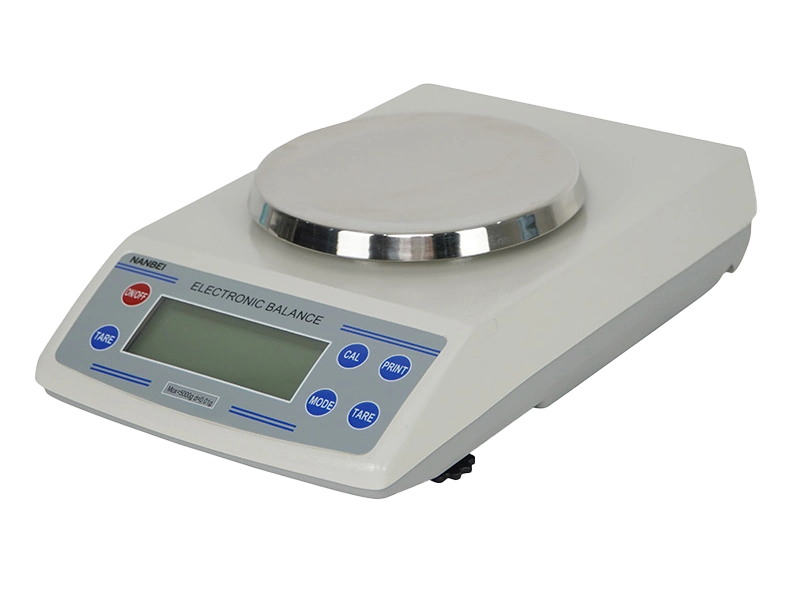
\includegraphics[width=2.2cm]{Images/candientu}};
			\node[rotate=0] (russell) at (1.5,0.5) {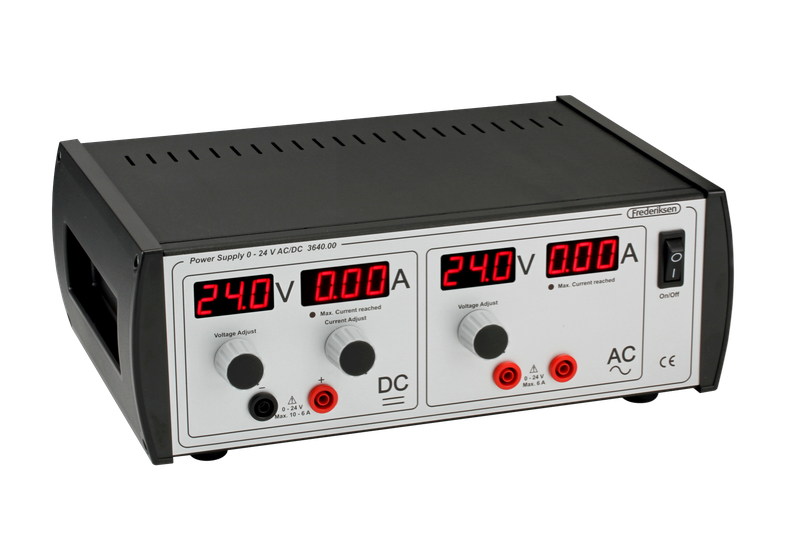
\includegraphics[width=2.8cm]{Images/bienthenguon}};
			\node[rotate=0] (russell) at (4,0.5) {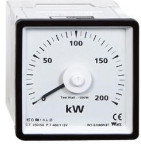
\includegraphics[width=1.5cm]{Images/oatke}};
			\node[rotate=0] (russell) at (6.5,1) {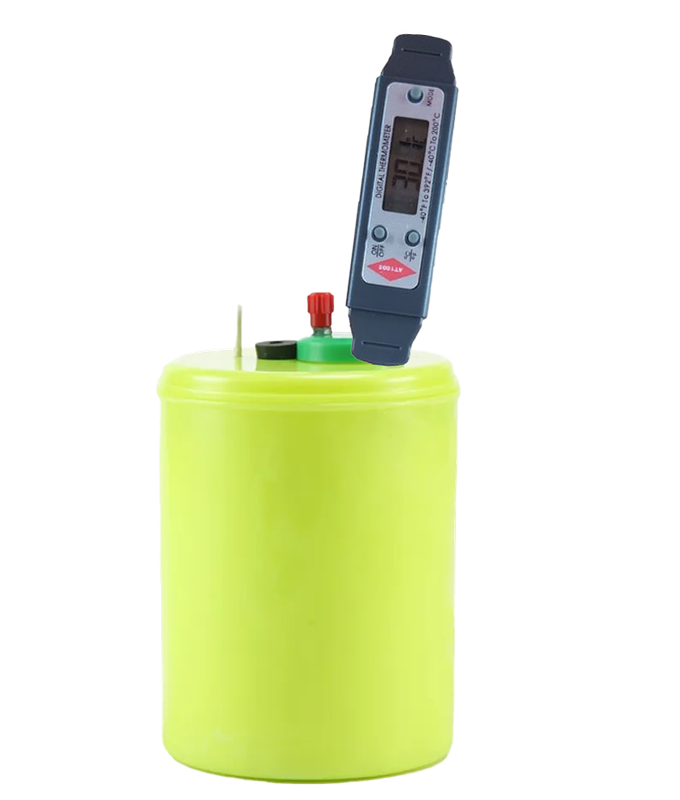
\includegraphics[width=2.6cm]{Images/nlkvank}};
			
			\node at (-1,2.5) {(5)};
			\node at (0.8,2.45) {(1)};
			\node at (4.5,-1) {(2)};
			\node at (7.5,-1.5) {(4)};
			\draw (-1,2) -- (-1,1);
			\draw (1,2) -- (1.5,1);
			\draw (4.35,-0.75) -- (4,-0.3);
			\draw (6.45,-0.65) -- (7.2,-1.25);
			\draw (6.5,2) -- (5.5,2.5);
			\node at (5.15,2.7) {(3)};
		\end{tikzpicture}
	\end{center}
	Hãy cho biết dụng cụ số (3) là
	\choice
	{Biến thế nguồn}
	{Cân điện tử}
	{Nhiệt lượng kế}
	{\True Nhiệt kế điện tử}
	\loigiai{
		Dụng cụ số (3) trong hình là nhiệt kế điện tử, dùng để đo nhiệt độ của nước.
	}
\end{ex}
\begin{ex} \nguon{2}
	\immini[thm]{Học sinh thả các thanh được nung nóng có khối lượng bằng nhau, được làm từ thép, đồng và nhôm vào ba nhiệt lượng kế có chứa cùng thể tích nước lạnh.  Nhiệt độ ban đầu của tất cả các thanh là như nhau và lớn hơn nhiệt độ của nước. Nhiệt độ ban đầu của nước trong tất cả các nhiệt lượng kế là như nhau. Khi cân bằng nhiệt thì nhiệt độ được ghi như hình bên. Chất có nhiệt dung riêng lớn nhất là
		\choice 
		{\True nhôm}
		{đồng}
		{thép}
		{chưa đủ căn cứ để kết luận}
	}	{ 
\includegraphics[width=7cm]{images/2024_05_26_41b28a481524728a6c0dg-26}}
	\loigiai{
		nhôm
	}
\end{ex}
\loai{Giải thích hiện tượng thực tế}
\begin{ex}
	Vào ban ngày và ban đêm thì hướng gió thổi thay đổi như thế nào ở các vùng ven biển?
	\choice
	{Ban ngày gió thổi từ Bắc tới Nam còn ban đêm gió thổi từ Nam tới Bắc}
	{\True Ban ngày gió thổi từ biển vào đất liền còn ban đêm gió thổi từ đất liền ra biển}
	{Ban ngày gió thổi từ Nam tới Bắc còn ban đêm gió thổi từ Bắc tới Nam}
	{Ban ngày gió thổi từ đất liền ra biển còn ban đêm gió thổi từ biển vào đất liền}
	\loigiai{
		Ban ngày, đất có nhiệt dung riêng thấp nên nóng lên nhanh hơn nước biển, khiến không khí trên đất liền nóng hơn. Do đó, gió thổi từ biển vào đất liền để thay thế lượng không khí tăng lên đó. Còn ban đêm, đất liền mất nhiệt nhanh chóng hơn biển, làm không khí trên đất liền lạnh đi và co lại, tăng mật độ và áp suất. Do đó, gió thổi từ đất liền ra biển để thay thế lượng không khí mất đi đó.
	}
	\haidong{2}
\end{ex}
\begin{ex} \nguon{4}
	Nếu ăn bánh ngọt ngay khi vừa đem ra khỏi lò nướng, phần vỏ bánh có thể không gây tổn hại gì đến bạn nhưng phần nhân sẽ làm bỏng lưỡi của bạn. Điều này được giải thích như thế nào?
	\choiceTF[t]
	{\True Phần nhân bánh, đặc biệt nếu có chứa nước hoặc các thành phần lỏng (như kem, mứt, hoặc nhân trái cây), có nhiệt dung riêng cao hơn}
	{\True Sau khi ra khỏi lò, vỏ bánh tiếp xúc trực tiếp với không khí bên ngoài nên nó nguội đi nhanh chóng}
	{Phần vỏ bánh được nướng ở nhiệt độ thấp hơn so với phần nhân}
	{Phần nhân bánh chứa ít nước hơn phần vỏ bánh nên nhiệt độ cao hơn}
	\loigiai{
		\begin{itemchoice}
			\itemch 
			\itemch 
			\itemch 
			\itemch 
		\end{itemchoice}
		\begin{itemize}
			\item ĐÚNG ĐÚNG SAI SAI
			\item  \textbf{Nhiệt dung riêng}: Nhiệt dung riêng của nước cao hơn so với các chất rắn trong vỏ bánh, giúp phần nhân giữ nhiệt lâu hơn.
			\item  \textbf{Khả năng cách nhiệt của vỏ bánh}: Vỏ bánh hoạt động như một lớp cách nhiệt, giữ nhiệt bên trong phần nhân.
			\item \textbf{Tốc độ tản nhiệt}: Vỏ bánh tản nhiệt nhanh hơn do tiếp xúc với không khí, trong khi phần nhân tản nhiệt chậm hơn do nằm bên trong.
			
			\item 	Ví dụ, nhiệt dung riêng của nước là khoảng $4186 \ J/kg.K$, trong khi nhiệt dung riêng của các chất rắn như bột mì là khoảng $1300 \ J/kg.K$. Điều này cho thấy phần nhân chứa nước có thể giữ lại nhiều nhiệt hơn.
			\item	Do đó, khi bạn ăn bánh ngay khi vừa ra khỏi lò, vỏ bánh đã nguội đi đủ để không gây bỏng, nhưng phần nhân bên trong vẫn còn rất nóng và có thể làm bỏng lưỡi của bạn. Để tránh bị bỏng, bạn nên để bánh nguội trong vài phút sau khi lấy ra khỏi lò, giúp nhiệt độ của cả vỏ và nhân giảm xuống mức an toàn để thưởng thức.
		\end{itemize}
	}
\end{ex}
\begin{ex} \nguon{2}
	\immini[thm]{ Để xác định nhiệt dung riêng của nước, có thể tiến hành thí nghiệm theo sơ đồ nguyên lí như hình bên}{
\includegraphics[width=7cm]{images/2024_05_26_41b28a481524728a6c0dg-19}}
	\choiceTF[t]
	{\True Biến áp nguồn có nhiệm vụ cung cấp cho mạch một hiệu điện thế}
	{Oát kế dùng để đo cường độ dòng điện của nguồn điện}
	{\True Nhiệt lượng tỏa ra trên dây điện trở bằng nhiệt lượng mà nước thu vào}
	{\True Nhiệt lượng kế ngăn cản sự truyền nhiệt của các chất đặt trong bình với môi trường bên ngoài} 
	\loigiai{
		\begin{itemize}
			\item [a)] Đúng
			\item [b)] Sai
			\item [c)] Đúng
			\item [d)] Đúng
		\end{itemize}
	}
\end{ex}
\begin{ex} \nguon{3}
	Những dụng cụ sau có trong thí nghiệm đo nhiệt dung riêng của nước. Các dụng cụ này có tên gọi là gì?
	\begin{center}
		\begin{tikzpicture}[scale=1.5,thick,>=stealth']
			\node[rotate=0] (russell) at (-0.5,0.5) {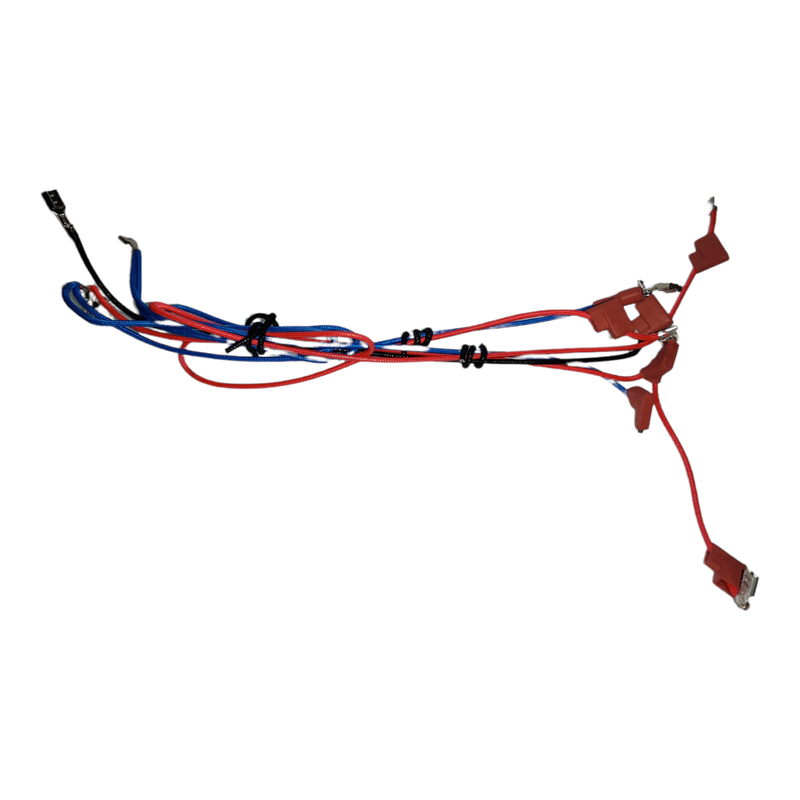
\includegraphics[width=2.2cm]{Images/daynoi1}};
			\node[rotate=0] (russell) at (1.5,0.5) {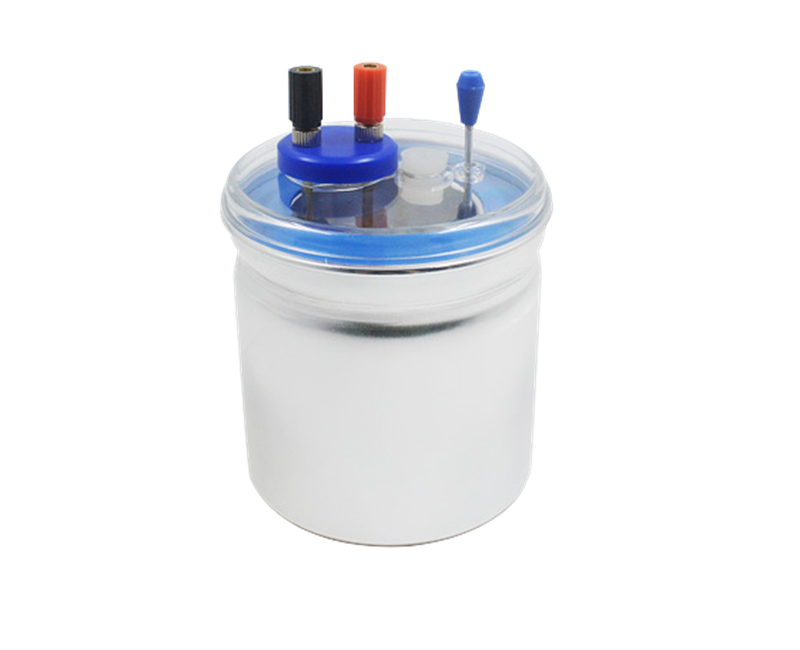
\includegraphics[width=3cm]{Images/nhietluongke1}};
			\node[rotate=0] (russell) at (3.5,0.5) {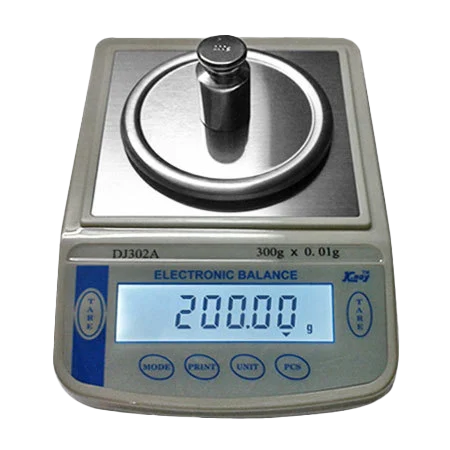
\includegraphics[width=2.5cm]{Images/candientu1}};
			\node[rotate=0] (russell) at (6.5,0.5) {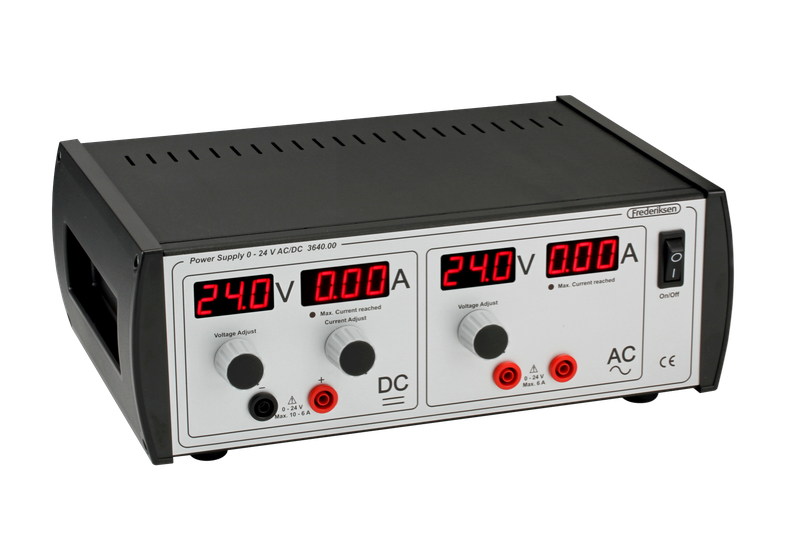
\includegraphics[width=3cm]{Images/bienthenguon}};
			
			\node at (-0.5,-1) {(1)};
			\node at (1.5,-1) {(2)};
			\node at (3.5,-1) {(3)};
			\node at (6.5,-1) {(4)};
		\end{tikzpicture}
	\end{center}
	
	\choiceTF[t]
	{\True Bộ phận số (1) là các dây nối}
	{Bộ phận số (2) là biến thế nguồn}
	{\True Bộ phận số (3) là cân điện tử}
	{Bộ phận số (4) là bình nhiệt lượng kế (có dây nung và que khuấy)}
	\loigiai{
		\begin{itemchoice}
			\itemch 
			\itemch Sai. 2 là nhiệt lượng kế.
			\itemch 
			\itemch Sai. 4 là biến thế nguồn
		\end{itemchoice}
	}
\end{ex}
\begin{ex} \nguon{2}
	Trên hình vẽ là đồ thị thu được từ thực nghiệm thể hiện sự phụ thuộc của nhiệt độ vào thời gian khi đun nóng một chất nào đó. Ban đầu chất ở trạng thái lỏng.
	\begin{center}
		\begin{tikzpicture}[scale=1.2,thick,>=stealth']
			\tkzDefPoints{0/0/o, 5/0/x, 0/4/y, 0.5/0/a, 2/2/b, 3.5/2/c, 4.5/3.5/d}
			\draw  [help  lines, xstep=0.5cm,ystep=0.5cm]  (0,0)  grid  (5,4);
			\tkzDrawSegments[->](o,x o,y)
			\tkzLabelPoint[below](o){$0$}
			\tkzLabelPoint[below right](x){$t$ (phút)}
			\tkzLabelPoint[above](y){$t\ (^\circ C)$}
			
			\foreach  \x  in  {1,2,...,4}
			{\pgfmathtruncatemacro{\label}{2*\x};
				\node[below]
				(\label) at (\x,0) {\label};
				\draw[fill=white](\x,0)circle(0.5pt);}
			
			\begin{scope}[shift={(0,-2)},rotate=0]
				\foreach  \y  in  {2,3,...,5}
				{\pgfmathtruncatemacro{\label}{20*\y};
					\node[left]
					(\label) at (0,\y) {\label};
					\draw[fill=white](0,\y)circle(0.5pt);}
			\end{scope}
			
			\tkzDrawSegments[very thick,red](a,b b,c c,d)
			\tkzDrawPoints[size=3,fill=white](a,b,c,d)
			\tkzLabelPoint[above left](a){$A$}
			\tkzLabelPoint[above](b){$B$}
			\tkzLabelPoint[above](c){$C$}
			\tkzLabelPoint[above](d){$D$}
			
		\end{tikzpicture}
	\end{center}
	\choiceTF[t]
	{\True Nhiệt độ sôi của chất lỏng là $80^\circ C$}
	{Nhiệt dung riêng của chất ở trạng thái lỏng và khí là như nhau}
	{Chất có nhiệt năng lớn nhất tại điểm C}
	{\True Chất có nhiệt năng nhỏ nhất tại điểm A}
	\loigiai{
		\begin{itemchoice}
			\itemch 
			\itemch 
			\itemch 
			\itemch 
		\end{itemchoice}
	}
\end{ex}
\begin{ex} \nguon{2}
	Trên đồ thị thể hiện kết quả đo nhiệt lượng $Q$, cần thiết để làm nóng $1 \ kg$ chất 1 và $1 \ kg$ chất 2, ở các giá trị nhiệt độ khác nhau của các chất này.
	\begin{center}
		\begin{tikzpicture}[scale=1.5,draw=Mapcolor, very thick, >=stealth']
			\tkzDefPoints{0/0/o, 3/0/x, 0/3/y}
			\draw  [help  lines, xstep=0.5cm,ystep=0.5cm]  (0,0)  grid  (3,3);
			\tkzDrawSegments[Mapcolor, very thick, ->](o,x o,y)
			\tkzLabelPoint[below](o){$0$}
			\tkzLabelPoint[below right](x){$t\ (^\circ C)$}
			\tkzLabelPoint[above](y){$Q\ (x10^3\ J)$}
			\draw[red,very thick] (0.5,0) -- (2.75,1.7);
			\draw[red,very thick] (0.4,0.13) -- (2.2,2.8);
			\foreach  \x  in  {1,2,...,4}
			{\pgfmathtruncatemacro{\label}{20*\x};
				\node[below]
				(\label) at (.5*\x,0) {\label};
				\draw[fill=white](.5*\x,0)circle(0.5pt);}
			
			\foreach  \y  in  {1,2,...,5}
			{\pgfmathtruncatemacro{\label}{10*\y};
				\node[left]
				(\label) at (0,.5*\y) {\label};
				\draw[fill=white](0,.5*\y)circle(0.5pt);}
			\node at (2.52,2.94) {1};
			\node at (2.98,2) {2};
		\end{tikzpicture}
	\end{center} 
	\choiceTF[t]
	{Nhiệt dung của hai chất là như nhau}
	{\True Nhiệt dung của chất thứ nhất lớn hơn nhiệt dung của chất thứ hai}
	{Để thay đổi nhiệt độ của $1 \ kg$ chất 1 thêm $20^\circ C$ cần lượng nhiệt $6000 \ J$}
	{\True Để thay đổi nhiệt độ của $1 \ kg$ chất 2 thêm $10^\circ C$ cần lượng nhiệt $3750 \ J$}
	\loigiai{
		\begin{itemchoice}
			\itemch 
			\itemch 
			\itemch 
			\itemch 
		\end{itemchoice}
	}
\end{ex}
%

